\section{B1. Approches techniques}

	L'intérêt du web offline est de permettre à un utilisateur d’utiliser ses applications habituellement connectées à internet (boite mail, streaming musical …) ou de consulter ses pages web préférées (casisbelli …), le tout, en étant hors-ligne. Cette technologie s’est principalement développée grâce à l’augmentation du nombre de smartphones et de tablettes. \\

	Afin de pouvoir utiliser un site web ou une application hors ligne, nous devons connaître l’état de connexion de l’utilisateur, c’est-à-dire, savoir s’il est connecté à internet ou non \textit{(pattern Message Endpoint)}. Cette étape est généralement réalisée à l’aide de fonctions de type javascripts en utilisant notamment : navigator.onLine. Une fois que nous avons pris connaissance de l’état de connexion de l’utilisateur, nous devons spécifier quelles sont et où sont situés les informations nécessaires afin d’afficher correctement le site internet ou le contenu de l’application. Cette étape passe généralement par la création d’un fichier appelé Cache Manifest et enregistré généralement sous le nom offline.manifest. Voici un exemple de fichier :\\

	CACHE MANIFEST\\
	angular.min.js\\
	bootstrap.min.js\\
	styles-perso.css\\
	jquery-1.4.min.js\\
	offline.js\\
	index.html\\
	exercices.html\\
	contact.html\\

	Il faut ensuite lier ce Cache Manifest à nos pages html de la manière suivante : \textit{$<html manifest="offline.manifest">$}\\

	Il est important de noter que les exemples donnés ci-dessus et par la suite de cette partie reposent sur l’utilisation de la technologie Application Cache. Il existe une autre technologie nommée Service Worker. \\

	Ensuite, il est important de stocker les données localement afin d’avoir accès aux données et de pouvoir utiliser correctement le site web ou l’application \textit{(pattern Message Store)}. \\

	Pendant l’utilisation, il est nécessaire de veiller à enregistrer les données régulièrement dans la base de données locale au risque de perdre des données dans le cas contraire. La solution la plus simple à mettre en place est la sauvegarde du DOM des pages web à l’aides des objets suivants :

	\begin{itemize}
		\item window.sessionStorage pour sauvegarder pendant la période de Session
		\item window.localStorage pour sauvegarder pour une période plus importante
	\end{itemize}

	Dans tous les cas, ces objets offrent le même type de fonction permettant d'accéder aux données, de sauvegarder ces dernières ou de les supprimer facilement.\\

	Une fois que la connexion à internet est rétablie, les données stockées en locale doivent être synchronisées avec le serveur distant \textit{(pattern Messaging)} \textit{(pattern Message Endpoint)} \textit{(pattern Message Filter)}. Il faut donc prévoir de créer une queue des données pour être cohérent avec l’évolution des données en mode hors ligne \textit{(pattern Resequencer)}. La transaction des données doit être vérifiée et réussie pour pouvoir passer à la transaction suivante \textit{(pattern Guaranteed Delivery)}. Si la connexion à internet coupe pendant une transaction, c’est comme ci elle n’avait pas été réalisée et doit donc être refaite lors d’une nouvelle connexion à internet. De plus, si des modifications ont été réalisées sur le serveur distant entre deux connexions, ces dernières vont être téléchargées vers le dossier de stockage local \textit{(pattern Shared Database)}.\\

	La figure~\ref{schema} explique de manière schématique les différentes grandes étapes de fonctionnement d'une application en web offline.

	\begin{figure}[h!]
		\centering
	  	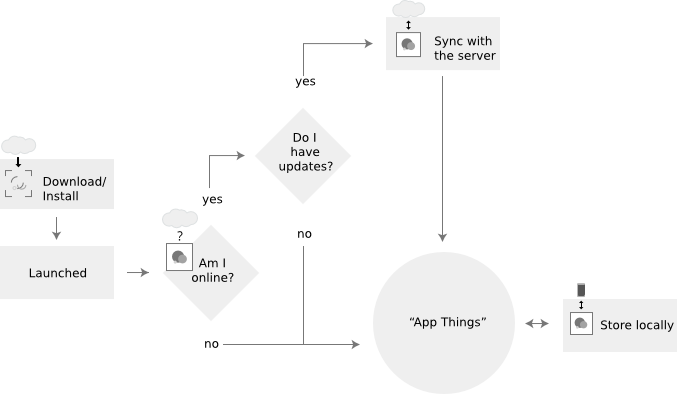
\includegraphics[width=18cm]{./images/schema.png}
	  	\caption{Schéma explicatif}
	  	\label{schema}
	\end{figure}

\section{B2. Solutions technologiques}

	Nous n'avons trouvé que deux solutions : 
	\begin{itemize}
		\item Application Cache;
		\item Service Worker.
	\end{itemize}

	Ainsi nous utiliserons ces deux solutions technologiques afin de réaliser les prototypes.

	\subsection{Application Cache}
		L'utilisation d'Application Cache permet à l'utilisateur de naviguer hors-ligne, il peut donc utiliser un site même s'il n'est pas connecté à internet. Les ressources sont mises en cache en locale et se chargent donc plus rapidement. Cela permet également de réduire la charge du serveur. Application Cache est directement intégré à HTML5, il sera donc plus facile à implémenter.

	\subsection{Service Worker}
		Service Worker est basé sur un script Javascript qui s'exécute en tâche de fond depuis une page internet. Il permet de contrôler la gestion des requêtes depuis le réseau. Il ne nécessite pas l'intervention d'un utilisateur pour s'exécuter.

\section{B3. Description technique}

	Détecter l'état de connexion à internet :
	\begin{itemize}
		\item offline.js
		\item failsafe.js
	\end{itemize}
	~\\

	Stockage des informations nécessaire à l’affichage :
	\begin{itemize}
		\item manifest
	\end{itemize}
	~\\
	
	Stockage des données :
	\begin{itemize}
		\item localForage
		\item localStorage
	\end{itemize}
	~\\

\section{B4. Benchmark}

	\begin{itemize}
		\item Functionality $->$ Interoperability
			\begin{itemize}
				\item Data exchangeability (data format-based)
			\end{itemize}
		\item Portability $->$ Adaptability
			\begin{itemize}
				\item System software environmental adaptability (adaptability to OS, network software and cooperated application software)
			\end{itemize}
		\item Reliability $->$ Recoverability
			\begin{itemize}
				\item Restoration effictiveness
			\end{itemize}
		\item Operation Time
		\item Number of Functions
	\end{itemize}
	~\\

\section{B5. Work Breakdown Structure}

	\begin{figure}[h!]
		\centering
		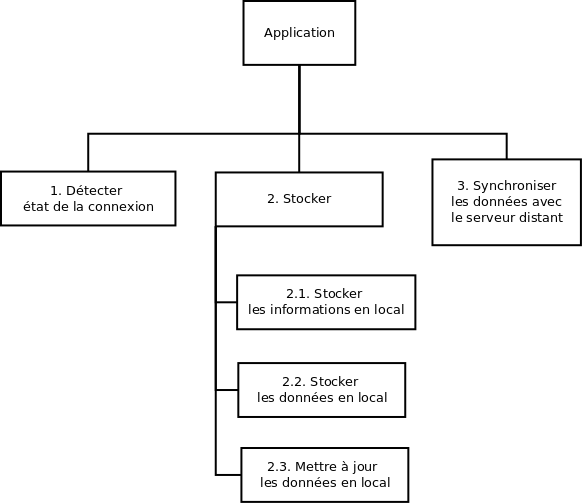
\includegraphics[width=18cm]{./images/wbs.png}
		\caption{Work Breakdown Structure}
	\end{figure}
